
\chapter{Results and Discussion}
\label{Chapter4}

\section{Results}

To evaluate the performance of this abundance estimation framework, we used both simulated readsets, in which the reference genome generating each read is known and the exact abundances can be calculated, and a real metagenomic sample generated artificially from even volumes of DNA of different organisms.

\subsection{Simulated Reads}

The following results were obtained running our method (with two different parameter sets), Bracken and DiTASiC on the read set from \textbf{[ref mende]}, a realistic simulated metagenome originally created for the assessment of performances of assembly algorithms.

The index used for the assignments includes 1267 genomes from 500 species, including the 193 genomes from 85 species in the read set. The same database was used to build indexes for Kraken and DiTASiC. Kraken's results have been further processed using the program Bracken, which redistributes reads assigned to internal nodes of the taxonomic tree to a fixed taxonomic rank (e.g. species, genus, etc.). The error estimations and false positive/negative rates are provided for every such rank till family, where the results of our model are virtually perfect. The results for Bracken at the genome level are not available since this tool is limited to the analysis at species level or above. Both a combination of $L_1$ and $L_2$ regularization penalties and a pure LASSO approach have been tested for our method, each providing results of different biological interest.

The table below contains the errors, calculated with the measures introduced in \textbf{[ref meth]}, of the three tools. In the row corresponding to false positive (resp. negative) rate, the first integer represents the number of variables (e.g. genomes, species, genera etc.), while the float between parentheses represents their estimated (resp. real) relative abundance. The figure \textbf{[ref fig]} shows the results of the tools compared to the ground truth, represented with black horizontal lines.

\begin{center}
\begin{tabular}{ c|c|p{2.2cm}|p{2.2cm}|p{2.3cm}|p{2.3cm}| }
Rank & Measure & $\lambda=1$ \newline $\alpha=0.01$ \newline (LASSO) & $\lambda=0.998$ \newline $\alpha=0.003$  \newline (E. Net) & Bracken & DiTASiC \\
\specialrule{.2em}{.1em}{.1em}
\multirow{5}{*}{Genome}
& MAE & 7.31e-4 & \textbf{6.33e-4} & NA & 8.52e-4 \\ \cline{2-6}
& RSS & \textbf{7.52e-4} & 9.32e-4 & NA & 2.26e-2 \\ \cline{2-6}
& FN \# (ab.) & 66 (1.06e-2) & \textbf{2} (\textbf{2.02e-4}) & NA & 32 (2.07e-2) \\ \cline{2-6}
& FP \# (ab.) & \textbf{32} (\textbf{5.60e-2}) & 89 (8.57e-2) & NA & 648 (3.22e-1) \\
\specialrule{.2em}{.1em}{.1em}
\multirow{5}{*}{Species}
& MAE & 3.20e-4 & \textbf{8.67e-5} & 1.52e-4 & 1.25e-3 \\ \cline{2-6}
& RSS & 3.84e-5 & \textbf{6.68e-6} & 2.79e-4  & 4.53e-2 \\ \cline{2-6}
& FN \# (ab.) & \textbf{0} (\textbf{0}) & \textbf{0} (\textbf{0}) & 1 (1.63e-2) & 0 (0) \\ \cline{2-6}
& FP \# (ab.) & \textbf{1} (\textbf{1.44e-4}) & 26 (1.36e-3) & 170 (9.73e-4) & 381 (6.08e-2) \\
\specialrule{.2em}{.1em}{.1em}
\multirow{5}{*}{Genus}
& MAE & 3.01e-4 & \textbf{4.98e-5} & 2.63e-4 & 1.97e-3 \\ \cline{2-6}
& RSS & 1.33e-5 & \textbf{1.16e-6} & 2.85e-4 & 5.45e-2 \\ \cline{2-6}
& FN \# (ab.) & \textbf{0} (\textbf{0}) & \textbf{0} (\textbf{0}) & 1 (1.63e-2) & 0 (0) \\ \cline{2-6}
& FP \# (ab.) & \textbf{0} (\textbf{0}) & 12 (3.62e-5) & 78 (3.23e-4) & 194 (1.06e-2) \\
\specialrule{.2em}{.1em}{.1em}
\multirow{5}{*}{Family}
& MAE & 3.22e-4 & \textbf{6.04e-5} & 3.85e-4 & 2.10e-3 \\ \cline{2-6}
& RSS & 1.35e-5 & \textbf{1.29e-6} & 2.86e-4 & 5.47e-2 \\ \cline{2-6}
& FN \# (ab.) & \textbf{0} (\textbf{0}) & \textbf{0} (\textbf{0}) & 1 (1.63e-2) & 0 (0) \\ \cline{2-6}
& FP \# (ab.) & \textbf{0} (\textbf{0}) & 7 (6.08e-6) & 42 (4.51e-5) & 108 (4.73e-3) \\
\hline
\end{tabular}
\end{center}

\begin{sidewaysfigure}
  \caption{Abundance profiles estimated by ProPhyle, Bracken and DiTASiC for the simulated dataset from \textbf{[ref mende]}.}
  \centering
    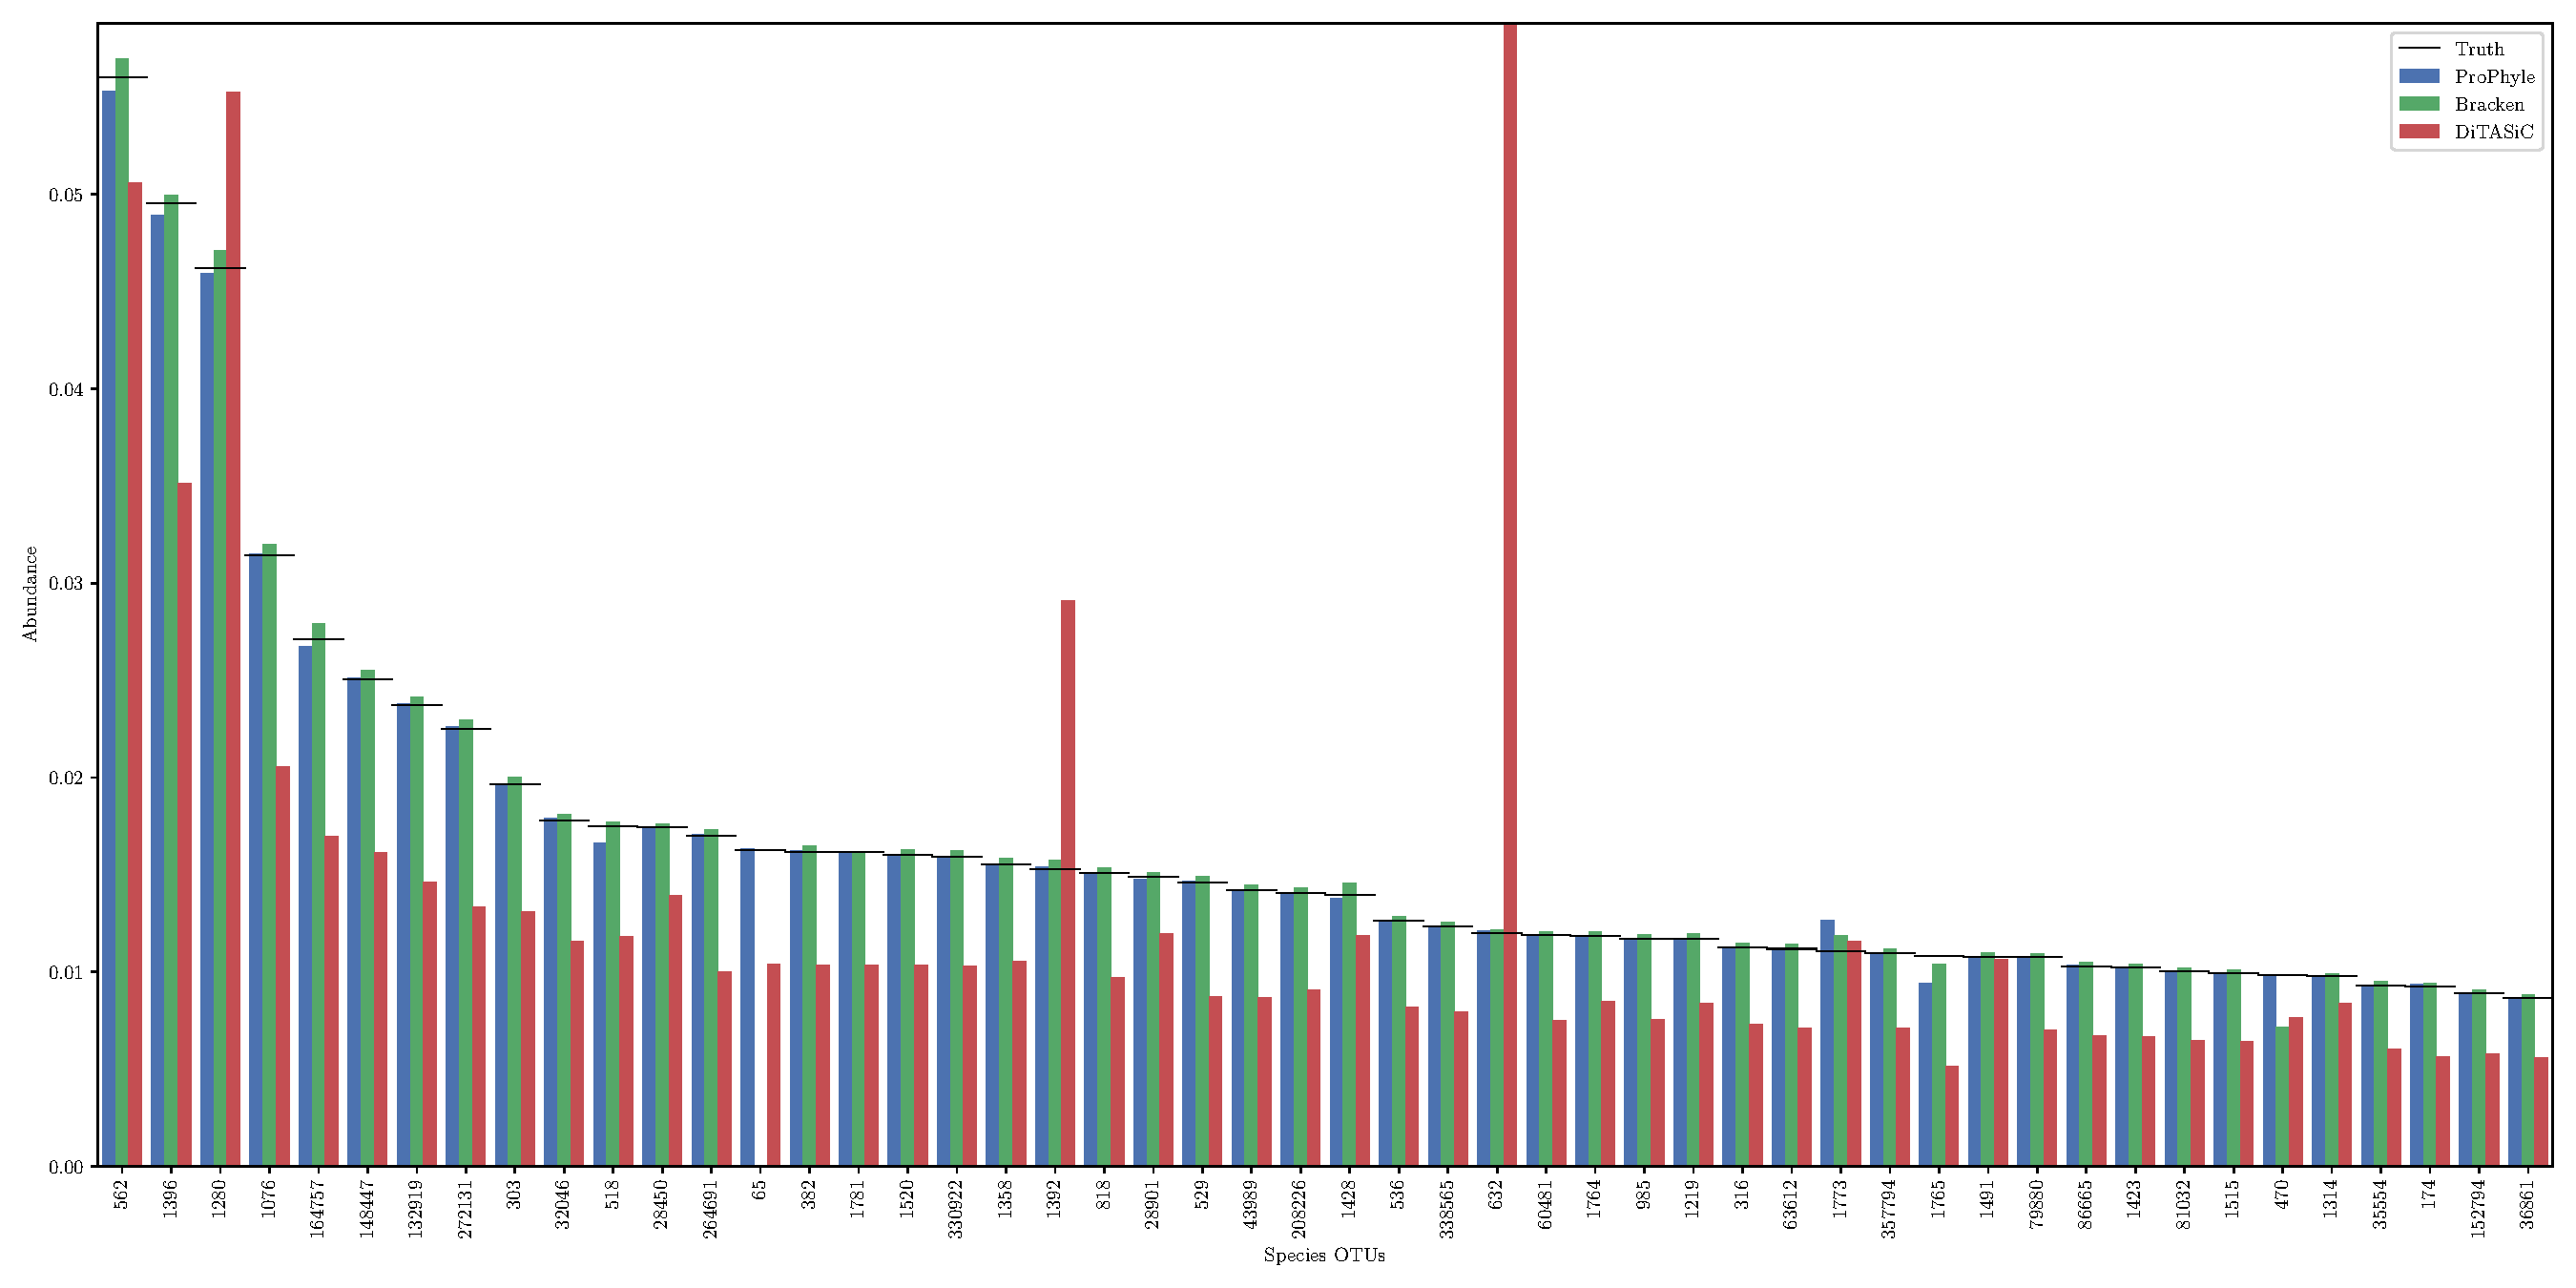
\includegraphics[width=1\textwidth]{Figures/ab_mende.pdf}
\end{sidewaysfigure}

Since the reference genomes were only a fraction of those used for real experiments, and the sample dataset was not nearly as complex as a real one, the best variable selection for ranks higher than genome is achieved by using only $L_1$ regularization (first column).
Nevertheless, introducing a very small coefficient for $L_2$ increases the overall precision and reduces the number of false negatives at genome level, probably thanks to the ``\textit{grouping effect}'' of the Elastic Net. This may be way more beneficial on real instances, where the optimal balance between $L_1$ and $L_2$ is expected to change substantially.

Our model outperforms both Bracken and DiTASiC for every error measure and every taxonomic rank, which makes us confident that the linear model is a better approximation for this problem compared to the Bayesian re-estimation performed by Bracken, and that the regularization effects are beneficial since they provide a satisfying variable selection compared to both Bracken and DiTASiC, the latter including basically half of the index in the output (648 FP over 1267 genomes in the index). Nevertheless, real metagenomic samples introduce challenges which may break the assumptions needed for the linear model to converge and provide meaningful estimations. While testing these conditions is not straightforward, since results on real samples may only be compared to those of other state-of-the-art tools which are not necessarily more accurate, we use a more realistic, ad-hoc simulation experiment to account for some of these challenges. Furthermore, we test our model on what is, to our knowledge, one of few metagenomic datasets for which the relative abundances of each component is known. We will see that even in this case it is hard to assess which part of the error is due to the DNA extraction protocol and the read sequencing process.

\subsection{Stress test}

In this experiment we simulated very complex metagenomes with low coverage from many different species. 10 samples were generated, each containing 500k read pairs of length 150bp originated from 250 different reference genomes. Since the abundance profile fits an exponential distribution, ~50 least abundant species (<e-5) of each sample only have 5 or less representative reads, and have been used to account for noise in the data (reads which originate from organisms not in the index, but which may match other relatives).

The index for this experiment was built upon all the ``reference'' and ``representative'' genomes in NCBI's RefSeq database, \dots

\subsection{Human Microbiome Project Mock Community}

In a real metagenomic scenario, where samples are collected directly from the environment and sequenced without prior isolation, it is extremely important to use an extensive database of reference genomes to reduce the number of reads which cannot be classified for lack of a close-enough representative genome. This has recently been explored in \textbf{[ref growrs]}, where the accuracy of the pipeline Kraken+Bracken was assessed for several versions of NCBI RefSeq, one of the most commonly used reference databases. For this reason, we have used the last version of RefSeq as of July 2018 to build the index of ProPhyle. Due to the size of the database, for which the construction of Kraken's index requires about 2.5TB of RAM and 11 days on a 64 cores compute node \textbf{[ref growrs]}, we have selected only the \textit{reference} and \textit{representative} genomes for each species, as defined in their website\footnote{\url{https://support.nlm.nih.gov/knowledgebase/article/KA-03578/en-us}}. This selection is mantained by NCBI to provide the highest diversity and quality of reference genomes. The total size of the reference database amounts to 30GB, and the resulting ProPhyle index requires 55GB of memory.

In addition to this issue, real metagenomic samples pose a great challenge to the performance benchmarks of classifiers, since the actual abundances in the sample are often unknown. To address this issue, we have used one of the few readsets for which a ground truth is provided: the pilot experiment for the Human Microbiome Project (HMP). The Human Microbiome Project is a research initiative to improve the understanding of the microbial flora involved in human health and disease, and in this pilot experiment they designed an even mixture of microbial DNA for which at least one reference was available in RefSeq at the time of the experiment. This provides a semi-realistic scenario for the benchmark of abundance estimation: while the data has been obtained by sequencing DNA with a physical machine, the composition of the sample is far from being realistic, since it only includes 22 organisms with uniformly distributed abundances.

Since some of the organisms which were used for the experiment have been removed from RefSeq, we only analyzed the performance at ranks species and higher. This poses another challenge to classification, since only a close relative genome is available in the reference database.

\begin{center}
\begin{tabular}{ c|c|c|c| }
Rank & Measure & Uniform & Adjusted \\ \hline
\multirow{5}{*}{Genome}
& RSS & 0.15 & 0.03 \\ \cline{2-4}
& FN \# (ab.) & 3 (0.14) & 3 (2.28e-6) \\ \cline{2-4}
& FP \# (ab.) & 5 (0.01) & 5 (0.01) \\
\specialrule{.2em}{.1em}{.1em}
\multirow{5}{*}{Species}
& RSS & 0.15 & 0.03 \\ \cline{2-4}
& FN \# (ab.) & 1 (0.05) & 1 (7.61e-7) \\ \cline{2-4}
& FP \# (ab.) & 3 (6.30e-3) & 3 (6.30e-3) \\
\specialrule{.2em}{.1em}{.1em}
\multirow{5}{*}{Genus}
& RSS & 0.15 & 0.03 \\ \cline{2-4}
& FN \# (ab.) & 0 (0) & 0 (0) \\ \cline{2-4}
& FP \# (ab.) & 1 (5.66e-3) & 1 (5.66e-3) \\
\hline
\end{tabular}
\end{center}

\section{Discussion}

The two experiments in the previous section show that the model is well defined and provides results comparable to the state-of-the art. Furthermore, compared to the work which inspired this\textbf{[ref gasic]}, the approach suggested is scalable to reference databases containing several thousands of genomes, as shown in \textbf{[ref realexp]}. This is possible thanks to the properties of the metagenomic classifier ProPhyle which produces accurate assignments in a fraction of the time required by traditional read alignment methods as those included in \textbf{[ref gasic]}.

The parametrization of the regularized linear model makes the method extremely flexible. As shown in \textbf{[ref simexp]}, by using a LASSO configuration it is possible to roughly estimate the composition of a sample, with virtually perfect results starting already at the species level; by introducing the $L_2$ penalty in the model and reducing the regularization weight, the method predicts extremely accurate abundances even at the genome level, at the price of introducing some false positives in the results.

The exponential growth of the reference databases still poses a threat to the scalability of the model, since simulating and assigning reads from the whole database may take weeks of computation in the near future. As we show in \textbf{[ref realexp]}, the method can still provide useful insights on the data when only few representatives for each species are included in the database, even if the genomes in the sample are not included.
